%% LaTeX-Beamer template for KIT design
%% by Erik Burger, Christian Hammer
%% title picture by Klaus Krogmann
%%
%% version 2.1
%%
%% mostly compatible to KIT corporate design v2.0
%% http://intranet.kit.edu/gestaltungsrichtlinien.php
%%
%% Problems, bugs and comments to
%% burger@kit.edu

\documentclass[18pt]{beamer}

\usepackage[utf8]{inputenc}
\usepackage[babel,german=quotes]{csquotes}
\usepackage{graphicx}
\usepackage{caption}
\usepackage{subfig}
\usepackage[right]{eurosym}
\usepackage{listings}

%% SLIDE FORMAT

% use 'beamerthemekit' for standard 4:3 ratio
% for widescreen slides (16:9), use 'beamerthemekitwide'

\usepackage{templates/beamerthemekit}
% \usepackage{templates/beamerthemekitwide}

%% TITLE PICTURE

% if a custom picture is to be used on the title page, copy it into the 'logos'
% directory, in the line below, replace 'mypicture' with the 
% filename (without extension) and uncomment the following line
% (picture proportions: 63 : 20 for standard, 169 : 40 for wide
% *.eps format if you use latex+dvips+ps2pdf, 
% *.jpg/*.png/*.pdf if you use pdflatex)

\titleimage{title}

%% TITLE LOGO

% for a custom logo on the front page, copy your file into the 'logos'
% directory, insert the filename in the line below and uncomment it

\titlelogo{titlelogo}

% (*.eps format if you use latex+dvips+ps2pdf,
% *.jpg/*.png/*.pdf if you use pdflatex)

%% TikZ INTEGRATION

% use these packages for PCM symbols and UML classes
% \usepackage{templates/tikzkit}
% \usepackage{templates/tikzuml}

% the presentation starts here

\title[C++ Workshop]{C++ Workshop}
\subtitle{1. Block, 27.04.2012}
\author{Markus Jung, Christian Käser, Robert Schneider}

\institute{}

\begin{document}

% change the following line to "ngerman" for German style date and logos
\selectlanguage{ngerman}

\AtBeginSection[]{%
	\begin{frame}
		\tableofcontents[sectionstyle=show/hide,subsectionstyle=hide/show/hide]
	\end{frame}
	\addtocounter{framenumber}{-1}% If you don't want them to affect the slide number
}

%title page
\begin{frame}
\titlepage
\end{frame}

%table of contents
\begin{frame}{Gliederung}
\tableofcontents
\end{frame}

%%%%%%%%%%%%%%%%%%%%%%%%%
% ADD OWN SECTIONS HERE %
%%%%%%%%%%%%%%%%%%%%%%%%%
%\include{cpp} % includes cpp.tex

\section{Praxis}

\begin{frame}{Towel-Day!}
	\begin{center}
		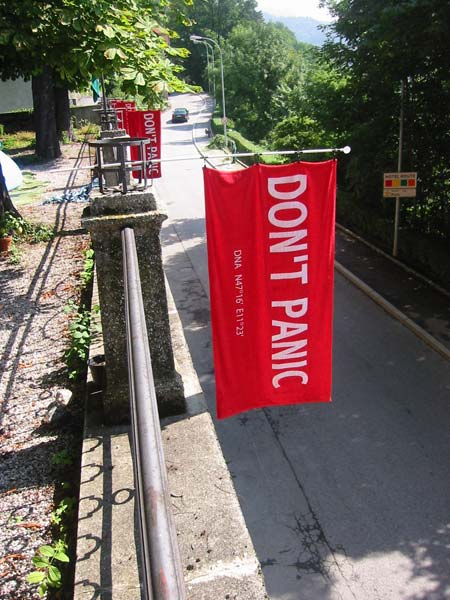
\includegraphics[height=0.8\textheight]{images/Towelday-Innsbruck.jpg}
	\end{center}
	
	\scriptsize
	\raisebox{4em}
	{
		Quelle: Wikimedia Commons
		CC-BY-SA 3.0 Beny Shlevich
	}
\end{frame}

\begin{frame}[fragile]{Praxis!}
	\begin{itemize}
		\item Aufgabe 1: Titel
		\item Aufgabe 2: Noch ein Titel
	\end{itemize}
	\ \\
	\ \\
	\large{\url{https://github.com/kit-cpp-workshop/workshop-ss12-04}} \\
	\ \\
	Aufgabenbeschreibungen und Hinweise: Siehe \verb|README.md|

\end{frame}


\end{document}
